\documentclass{sintefbeamer}

% packages, font, color, and newcommands
\usepackage{amsfonts, amsmath, oldgerm, lmodern, bm}
% \usepackage[font={footnotesize}]{caption}
\usepackage{natbib}
\usepackage{url}
\usepackage{tikz}
\usepackage{amssymb}
\usepackage{amsmath}
\usepackage{amsthm}
\usepackage{mathrsfs}
\usepackage{empheq}
\usepackage{mdframed}
\usepackage{bm}
\usepackage{animate}
\usepackage{xcolor,colortbl}
\usepackage{graphicx}
\bibliographystyle{apalike}
\usefonttheme{serif}
\usetikzlibrary{calc}

\title{Nearest particule microstructure in rising monodisperse suspensions of drops\break}

\author{\href{http://basilisk.fr/sandbox/fintzin/Rising-Suspenion/RS.c}{\underline{N. Fintzi}\footnote{IFP \'Energies Nouvelles, Lyon, France}$^{,2}$}, JL. Pierson$^1$ and S. Popinet\footnote{CNRS \& Sorbonne Universit\'e, Paris, France}}
% \date{Created on May 22, 2022}

\titlebackground{image/3D/P_PHI_5.png}

% document body
\addtobeamertemplate{navigation symbols}{}{%
    \usebeamerfont{footline}%
    \usebeamercolor[fg]{footline}%
    % \hspace{1em}%
    % \vspace{1em}%
    \insertframenumber/\inserttotalframenumber
}
\usepackage{stmaryrd}

\usepackage{amsmath}


\begin{document}
\maketitle

\begin{frame}
  \frametitle{Industrial context}
  \underline{Emulsions and bubbly flows are ubiquitous in chemical engineering processes:}
  \begin{itemize}
    \item Liquid-liquid separation
    \item Bubble column reactors
  \end{itemize}
  \vfill
  \underline{In all these processes we need to: }
  \begin{itemize}
    \item Predict global hydrodynamics in dispersed bubbly flows and emulsions (interphase forces etc\ldots).
    \begin{itemize}
      \item Models for the interphase drag forces.
      \item Models for the interphase Reynolds stress.
      \item Models for size distributions and coalescence/breakup:
      \begin{itemize}
        \item Describe the interactions between pairs of droplets
        \item Predict the interaction frequency
        \item Predict the film drainage time
        \item etc...
      \end{itemize}
    \end{itemize}
  \end{itemize}

  \vfill
\end{frame}

\begin{frame}
  {A multiscale problem}
  \begin{tikzpicture}
    \node (img0) at (-0.1\textwidth,-0.35\textwidth) {
\includegraphics[height=0.1\textwidth]{image/logo.png} http://basilisk.fr};
    \node (img1) at (0,0) {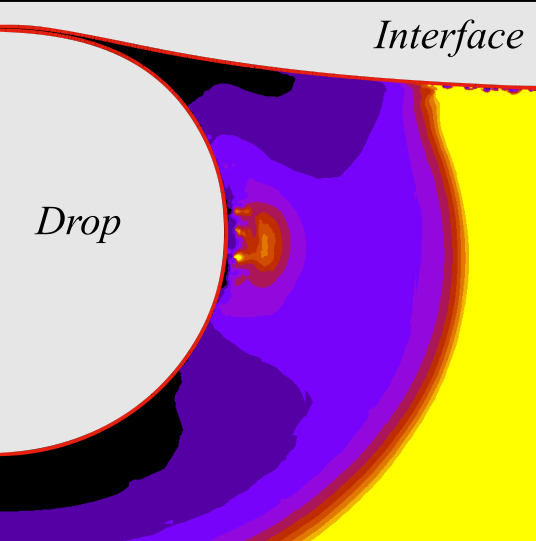
\includegraphics[height=0.25\textwidth]{image/film_drainage.png}};
    \node (img2) at (0.35\textwidth,-0.1\textwidth) {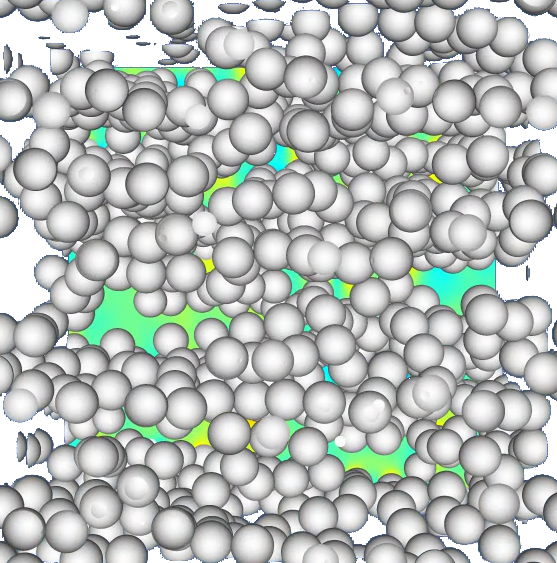
\includegraphics[height=0.25\textwidth]{image/700drop.png}};
    \node (ttx) at (0.35\textwidth,0.1\textwidth){Coalescence closure};
    \node (img3) at (0.7\textwidth,0) {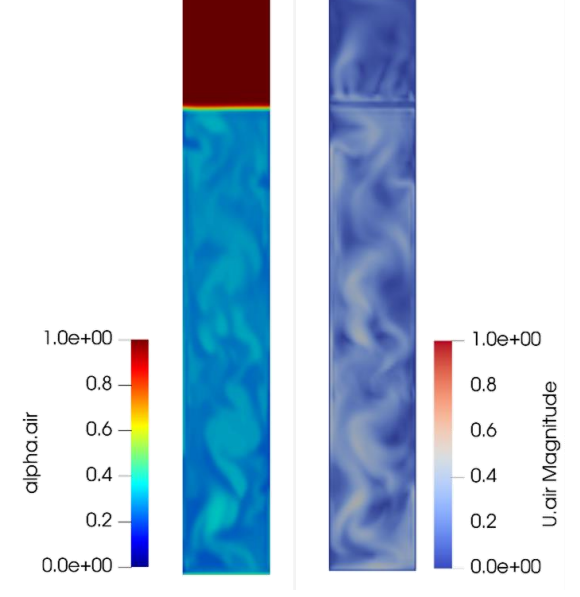
\includegraphics[height=0.25\textwidth]{image/Euler_Euler.png}};
    \node[below,text width=0.3\textwidth] (imgC) at (img1.south) {Film scale: 
    \begin{itemize}
      \item Film drainage time % (Naanouh  Paul-Peter PhD. ) 
    \end{itemize}};
    \node[below,text width=0.3\textwidth] (imgC) at (img2.south) {Inter-particule scale: 
    \begin{itemize}
      \item Interaction dynamics % (Fintzi Nicolas PhD. ) 
    \end{itemize}};
    \node[below,text width=0.3\textwidth] (imgC) at (img3.south) {Process scale:
    \begin{itemize}
      \item Process optimization % (Landal Kamel PhD. ) 
    \end{itemize}
    };
    \draw[->,very thick] (img1) -- (ttx.west);
    \draw[->,very thick] (img2.north) -- (ttx);
    \draw[->,very thick] (ttx.east) -- (img3);
    \draw[red,very thick] (img2.south west) rectangle(img2.north east);
  \end{tikzpicture}
\end{frame}

\begin{frame}
  {In Nicolas' PhD we focus on three aspects of the problem:}
  \Large
  \begin{enumerate}
    \item Mathematical modeling of \textbf{averaged dispersed two-phase flows} with a kinetic-theory like model. 
    \begin{itemize}
      \item What is the difference with classical solid particule models? (R. Jackson 1997, D.Z. Zhang and A. Prosperetti 1997)
      \item Does surface tension play a role in the conservation equations? 
      \item How to model non-spherical and deforming particules?
    \end{itemize}  
    \item DNS of buoyant emulsions to close this mathematical model (Reynolds stress model and drag force model \ldots). 
    % \begin{itemize}
    %   \item Provide closure terms for the averaged Navier Stokes equations such as the Drag force, Reynolds Stresss, Particule-fluid-Particule stress \ldots 
    % \end{itemize}
    \item[\textcolor{red}{3.}] We use the Nearest Particule Statistics framework to explain qualitatively and quantitatively the \textbf{average interaction behaviour} between droplet pairs within a buoyant emulsion. 
    % \begin{itemize}
      % \item How to model theoretically the pair properties ? 
      % \item How to define an interaction within space and time ? 
    % \end{itemize} 
  \end{enumerate}
  This presentation focuses on (\textcolor{red}{3.})
\end{frame}


\section{Direct Numerical Simulation (DNS) of buoyant emulsions}
\section*{}

\begin{frame}
\frametitle{Direct Numerical Simulation of buoyant emulsions}
\begin{columns}
  \column{0.6\textwidth}
\underline{Simulation set up :} 
\begin{itemize}
\item Tri-periodic boundary conditions.
\item Buoyancy only.
\item \textbf{Mono-disperse} distribution of droplet size.
\item We prevent (VOF) coalescence using a special algorithm 
  (\href{http://basilisk.fr/src/no-coalescence.h}{no-coalescence.h})
\item Free Software: \url{http://basilisk.fr}
\end{itemize}

\begin{figure}
  \caption{Snapshot of a simulation at $T_g = 300$ for $\phi = 0.01$, $Ga = 75$, $\mu_r = 0.1$ and $N_b = 125$. In white, the interfaces ; the background color map corresponds to the pressure field. The grid represents the different parallel cores.
  }
\end{figure}
\column{0.5\textwidth}
\centering
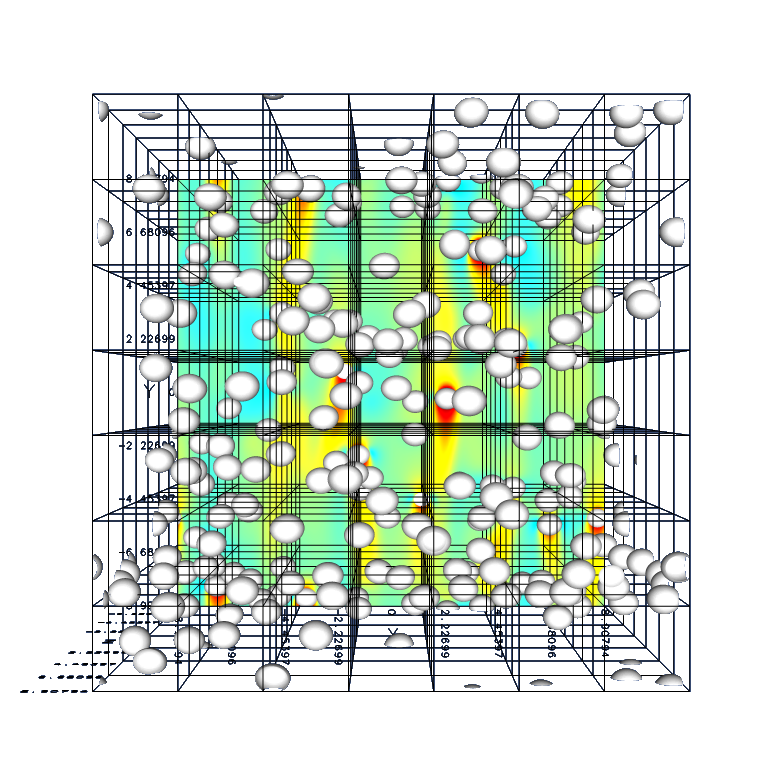
\includegraphics[width =  1.1\textwidth]{image/PHI_01_Ga_75.png}
\end{columns}
\end{frame}

\begin{frame}
  \frametitle{Direct Numerical Simulation of buoyant emulsions}
  \begin{columns}
    \column{0.6\textwidth}
  \underline{Dimensionless parameters:} 
  \begin{itemize}
    \item \textit{Galileo} number: $Ga =\frac{\sqrt{\rho \Delta\rho gD^3}}{\mu} \in [5, 100]$
    \item \textit{Bond} number: $Bo = \frac{\Delta \rho g D^2}{\sigma} = 0.2$ 
    \item Volume fraction of dispersed phase: $\phi = [0.01;0.2]$. 
    \item Density and viscosity ratio, $\rho_r=1.11$ and $\lambda= 10,1,0.1$. 
  \end{itemize}
  
\begin{figure}
  \caption{Snapshot of a simulation at $T_g = 300$ for $\phi = 0.01$, $Ga = 75$, $\mu_r = 0.1$ and $N_b = 125$. In white, the interfaces ; the background color map corresponds to the pressure field. The grid represents the different parallel cores.
  }
\end{figure}
\column{0.5\textwidth}
\centering
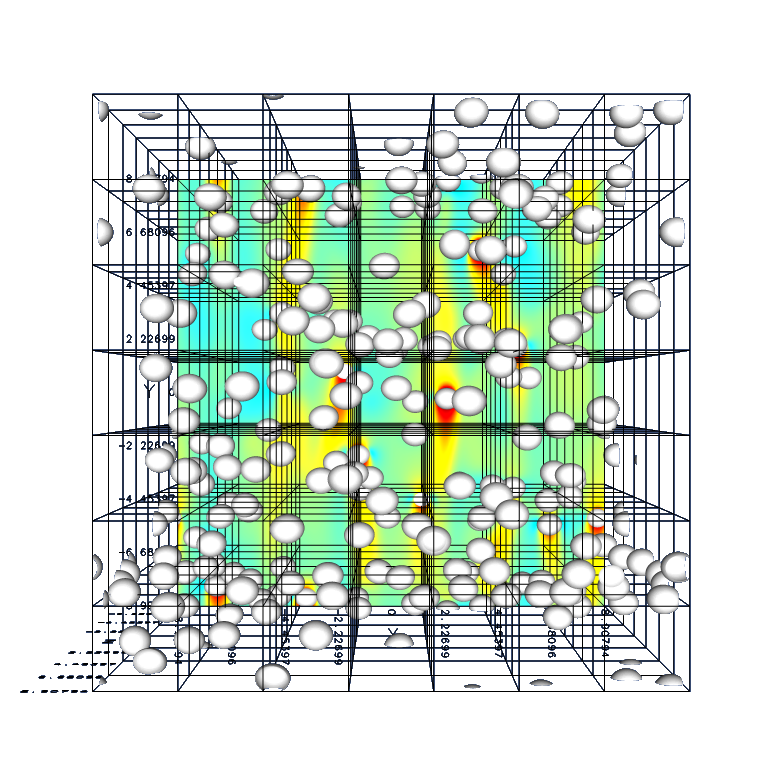
\includegraphics[width =  1.1\textwidth]{image/PHI_01_Ga_75.png}
  \end{columns}
\end{frame}


\begin{frame}
  \frametitle{Drag coefficient model for viscous droplet emulsions}
  \begin{figure}[h!]
    \centering    
    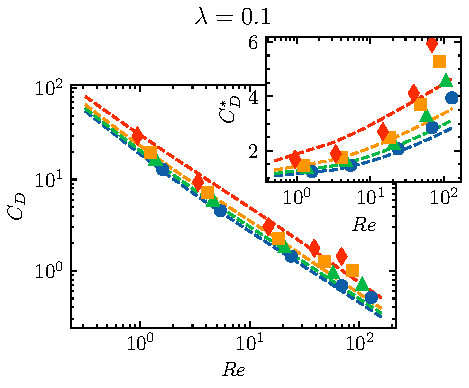
\includegraphics[height = 0.23\textwidth]{image/HOMOGENEOUS_final/CA/Cp_l_0.pdf}
    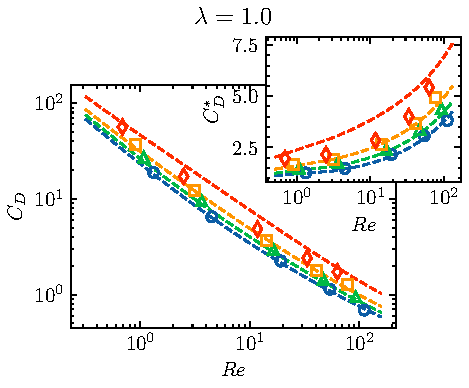
\includegraphics[height = 0.23\textwidth]{image/HOMOGENEOUS_final/CA/Cp_l_1.pdf}
    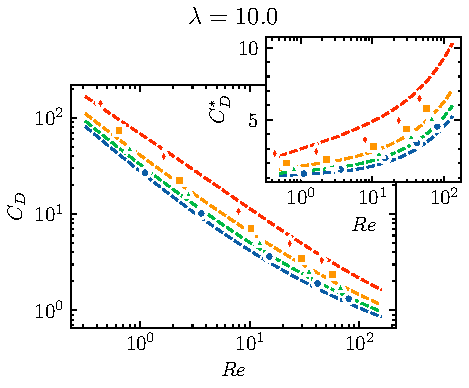
\includegraphics[height = 0.23\textwidth]{image/HOMOGENEOUS_final/CA/Cp_l_10.pdf}
    \caption{
        Drag coefficient $C_p$ in term of the Reynolds number $Re$.  
        The symbols correspond to different volume fractions. 
    }
    \label{fig:Cp}
\end{figure}
% \footnotesize
\begin{equation*}
  C_d(Re,\phi,\textcolor{red}{\lambda})
  = \frac{  \textcolor{red}{\lambda}   (C_D)_\text{Solid}+ (C_D)_\text{Bubbles}}
  {1+\textcolor{red}{\lambda}} 
  \left[
    \frac{1}{(1- \phi)^{n(\textcolor{red}{\lambda})-3}}
  \right]
\end{equation*}
\begin{itemize}
  % \item Creation of a new model which takes in account the viscosity ratio : \textcolor{red}{$\lambda$}. 
  \item $(C_D)_\text{Solid}$ is the drag coefficient on an isolated solid sphere and $(C_D)_\text{Bubbles}$ the drag coefficient on a shear-free bubble
  \item From Richardson and Zaki (1954) and others: $n(\lambda) = 4.5 \left[\frac{2/3 +\lambda }{\lambda +1}\right]$ 
\end{itemize}

\end{frame}

\section{Description of the interactions}
\section*{}


\begin{frame}
  \frametitle{How to describe pair interactions and microstructure?}
  % To better model the film drainage problem we need a clear understanding of How the interactions between droplets works. 
  
  \textbf{Nearest Particule Statistics (Duan Z. Zhang, JFM, 2021): }
  \begin{definition}
    \begin{itemize}
      \item Let $\mathscr{C} =\left\{\textbf{x}_1, \textbf{r}, \textbf{w},a\right\}$ be the vector containing the position of a particule $\textbf{x}_1$, its nearest neighboring particule relative position $\textbf{r}$, the relative velocity \textbf{w} and the age of the pair time interaction $a$.
      \item Then, $P_{nst}(\textbf{x},\textbf{r},\textbf{w},a) $ is the probability of finding a particule at \textbf{x} with its nearest neighboring particule at \textbf{r} with a relative velocity of \textbf{w} and an age $a$. 
    \end{itemize}
  \end{definition}

  \begin{align*}
    P_{nst}(\textbf{x},\textbf{r},\textbf{w},a)
    &= \int \Pi(\textbf{x},\textbf{r},\textbf{w},a) d\CC\\
    \textbf{f}^\text{nst} P_{nst}(\textbf{x},\textbf{r},\textbf{w},a)
    &= \int \textbf{f} \Pi(\textbf{x},\textbf{r},\textbf{w},a) d\CC
  \end{align*}
  \begin{itemize}
    \item 
    where $\Pi = 1$ if and only if a particule is present at \textbf{x} with its nearest neighbor at \textbf{r} = $\textbf{y}-\textbf{x}$, having an age of $a$ with relative velocity \textbf{w}. 
    \item $\textbf{f}$ can be a particule property or an Eulerian property of the continuous phase. 
  \end{itemize}
\end{frame}


\begin{frame}
  \frametitle{Nearest pair Probability Density Function}

  \begin{columns}
    \column{0.7\textwidth}
    \centering
    \begin{tabular}{cccc}
      &
      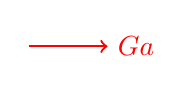
\begin{tikzpicture}[color=red]
        \draw[thick,->] (0,0) -- (1,0)node[right]{$Ga$};
      \end{tikzpicture}& & \\ 
        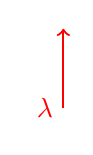
\begin{tikzpicture}[color=red]
          \draw[thick,<-] (0,0) -- (0,-1)node[left]{$\lambda$};
        \end{tikzpicture} 
        &
        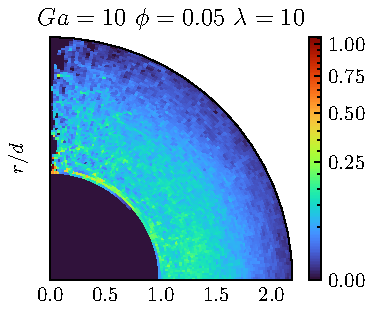
\includegraphics[height=0.3\textwidth]{image/HOMOGENEOUS_NEW/Dist/Pnst_l_10_Ga_10_PHI_0_05.pdf}  &
        % 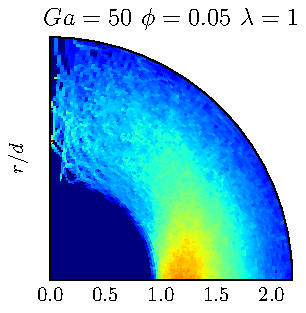
\includegraphics[height=0.3\textwidth]{image/HOMOGENEOUS_NEW/Dist/Pnst_l_1_Ga_50_PHI_0_05.pdf} &
        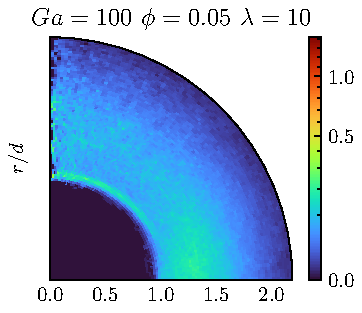
\includegraphics[height=0.3\textwidth]{image/HOMOGENEOUS_NEW/Dist/Pnst_l_10_Ga_100_PHI_0_05.pdf} 
        \\
         &
          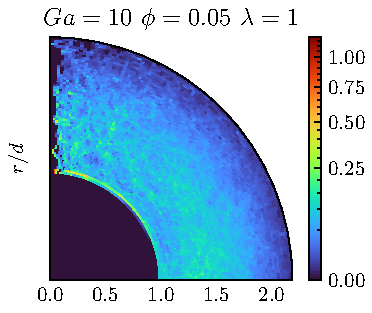
\includegraphics[height=0.3\textwidth]{image/HOMOGENEOUS_NEW/Dist/Pnst_l_1_Ga_10_PHI_0_05.pdf} &
        % 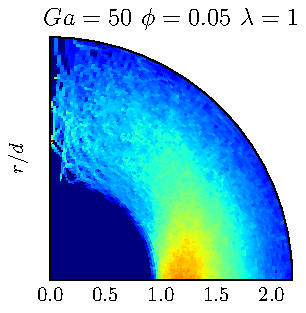
\includegraphics[height=0.3\textwidth]{image/HOMOGENEOUS_NEW/Dist/Pnst_l_1_Ga_50_PHI_0_05.pdf}&
        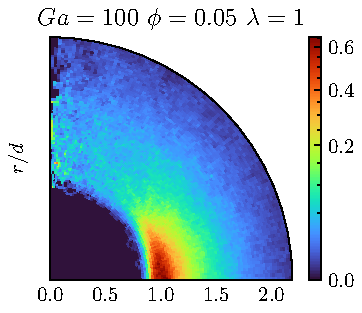
\includegraphics[height=0.3\textwidth]{image/HOMOGENEOUS_NEW/Dist/Pnst_l_1_Ga_100_PHI_0_05.pdf}\\
      \end{tabular}

      \column{0.3\textwidth}
      \begin{figure}
        \caption{Plots of $P_{nst} (\textbf{r})$ for different $Ga$ and $\phi$.}
      \end{figure}
    
    \begin{itemize}
      \item Drafting-Kissing-Tumbling mechanism for low $\lambda$ and high $Ga$. 
    \end{itemize}
  \end{columns}
  $\to$ The viscosity ratio $\lambda$ greatly influences the microstructure
\end{frame}

\begin{frame}
  \frametitle{Consequence on the particule arrangements}

  \begin{figure}[h!]
    \centering
    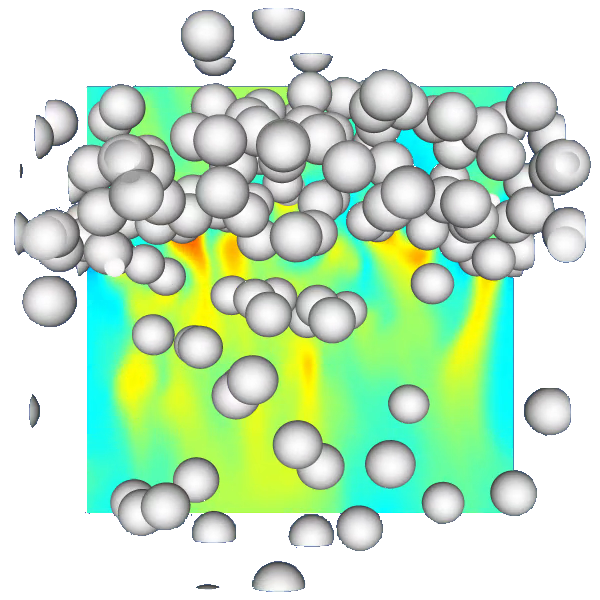
\includegraphics[width=0.45\textwidth]{image/HOMOGENEOUS_NEW/P_PHI_5_l_10_Ga_100.png}
    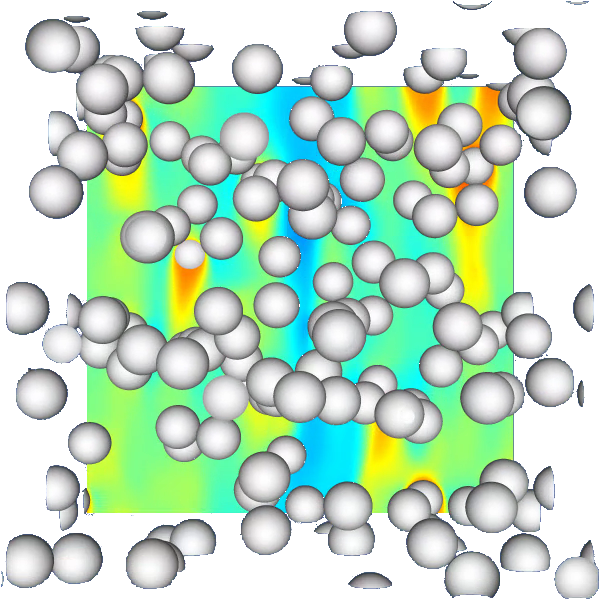
\includegraphics[width=0.45\textwidth]{image/HOMOGENEOUS_NEW/P_PHI_5_l_1_Ga_100.png}
 %    \includegraphics[width=0.45\textwidth]{image/HOMOGENEOUS_NEW/Ga_100_phi_005_l_10.png}
    \caption{Snapshot of a simulation at $t^* = 150$ for $\phi=0.05$ and $Ga=100$.
      Color map: values of the vertical component of the velocity field on the vertical plane at $z=0$.
      \break
    (left)  $\lambda = 1$.
    (right)  $\lambda = 10$.
    }
    \label{fig:images}
 \end{figure}

\end{frame}


\begin{frame}
  {A concise way to describe the microstructure}
\footnotesize
  We use the second moment of the pair distribution: 
  \begin{align*}
    \textbf{R} = \int \textbf{rr} P_{nst}(\textbf{r}) d\textbf{r}
    &&
    \textbf{A} = 
    \textbf{R} - \frac{1}{3}(\textbf{R}: \bm\delta) \bm\delta
  \end{align*}

%   \begin{figure}
%   \centering
%   \begin{tikzpicture}
    
%   \foreach \i in {1,...,5} {
%   \pgfmathsetmacro{\x}{rnd*0.7}
%   \pgfmathsetmacro{\y}{rnd*0.3}
%   \draw[fill=gray] ($(\x,\y)$) circle (0.1);
%   }
%   \foreach \i in {1,...,5} {
%   \pgfmathsetmacro{\x}{rnd*0.7}
%   \pgfmathsetmacro{\y}{rnd*0.3}
%   \draw[fill=gray] ($(\x+2,\y)$) circle (0.1);
%   }
%   \foreach \i in {1,...,5} {
%   \pgfmathsetmacro{\x}{rnd*0.6}
%   \pgfmathsetmacro{\y}{rnd*0.4}
%   \draw[fill=gray] ($(\x+1,\y-1)$) circle (0.1);
%   }
%   \foreach \i in {1,...,5} {
%   \pgfmathsetmacro{\x}{rnd*0.6}
%   \pgfmathsetmacro{\y}{rnd*0.4}
%   \draw[fill=gray] ($(\x-1,\y-1)$) circle (0.1);
%   }
%   \draw (1,-1)node[below]{$\text tr(\textbf {R}) \ll 1$};

%     \foreach \i in {1,...,20} {
%       \pgfmathsetmacro{\x}{rnd*4}
%       \pgfmathsetmacro{\y}{rnd*2}
%       \draw[fill=gray] ($(\x+5,\y-1)$) circle (0.1);
%       }
%       \draw (6.5,-1)node[below]{$\text tr(\textbf {R})/r_m^2 < 1$};
%     \end{tikzpicture}
%     \hfill
% \end{figure}
\begin{figure}
  \centering
  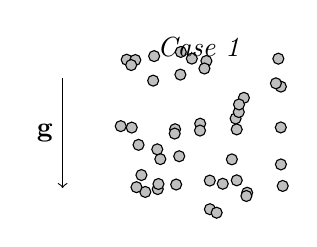
\begin{tikzpicture}[scale=0.7]
  \draw[->] (-1,2.5)--++(0,-2)node[midway, left]{$\textbf{g}$};
  \foreach \i in {1,...,5} {
  \pgfmathsetmacro{\x}{rnd}
  \pgfmathsetmacro{\y}{rnd}
  \draw[fill=gray!50] ($(\x,\y)$) circle (0.1);
  }
  \foreach \i in {1,...,5} {
  \pgfmathsetmacro{\x}{rnd}
  \pgfmathsetmacro{\y}{rnd}
  \draw[fill=gray!50] ($(\x+1,\y)$) circle (0.1);
  }
  \foreach \i in {1,...,5} {
  \pgfmathsetmacro{\x}{rnd}
  \pgfmathsetmacro{\y}{rnd}
  \draw[fill=gray!50] ($(\x+2,\y)$) circle (0.1);
  }
  \foreach \i in {1,...,5} {
      \pgfmathsetmacro{\x}{rnd}
      \pgfmathsetmacro{\y}{rnd}
      \draw[fill=gray!50] ($(\x+1,\y+1)$) circle (0.1);
  }
  \foreach \i in {1,...,5} {
  \pgfmathsetmacro{\x}{rnd}
  \pgfmathsetmacro{\y}{rnd}
  \draw[fill=gray!50] ($(\x+2,\y+1)$) circle (0.1);
  }
  \foreach \i in {1,...,5} {
  \pgfmathsetmacro{\x}{rnd}
  \pgfmathsetmacro{\y}{rnd}
  \draw[fill=gray!50] ($(\x,\y+1)$) circle (0.1);
  }
  \foreach \i in {1,...,5} {
      \pgfmathsetmacro{\x}{rnd}
      \pgfmathsetmacro{\y}{rnd}
      \draw[fill=gray!50] ($(\x+1,\y+2)$) circle (0.1);
  }
  \foreach \i in {1,...,5} {
  \pgfmathsetmacro{\x}{rnd}
  \pgfmathsetmacro{\y}{rnd}
  \draw[fill=gray!50] ($(\x+2,\y+2)$) circle (0.1);
  }
  \foreach \i in {1,...,5} {
  \pgfmathsetmacro{\x}{rnd}
  \pgfmathsetmacro{\y}{rnd}
  \draw[fill=gray!50] ($(\x,\y+2)$) circle (0.1);
  }
  \draw (1.5,3.4)node[below]{\textit{Case 1}};
\end{tikzpicture}
\hfill
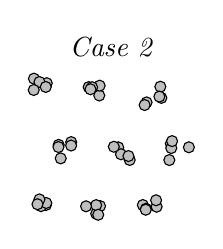
\begin{tikzpicture}[scale=0.7]
  \foreach \i in {1,...,5} {
  \pgfmathsetmacro{\x}{rnd*0.4}
  \pgfmathsetmacro{\y}{rnd*0.4}
  \draw[fill=gray!50] ($(\x,\y)$) circle (0.1);
  }
  \foreach \i in {1,...,5} {
  \pgfmathsetmacro{\x}{rnd*0.3}
  \pgfmathsetmacro{\y}{rnd*0.3}
  \draw[fill=gray!50] ($(\x+1,\y)$) circle (0.1);
  }
  \foreach \i in {1,...,5} {
  \pgfmathsetmacro{\x}{rnd*0.3}
  \pgfmathsetmacro{\y}{rnd*0.3}
  \draw[fill=gray!50] ($(\x+2,\y)$) circle (0.1);
  }
  \foreach \i in {1,...,5} {
      \pgfmathsetmacro{\x}{rnd*0.5}
      \pgfmathsetmacro{\y}{rnd*0.5}
      \draw[fill=gray!50] ($(\x+0.5,\y+1)$) circle (0.1);
  }
  \foreach \i in {1,...,5} {
      \pgfmathsetmacro{\x}{rnd*0.4}
      \pgfmathsetmacro{\y}{rnd*0.4}
      \draw[fill=gray!50] ($(\x+2.5,\y+1)$) circle (0.1);
  }
  \foreach \i in {1,...,5} {
      \pgfmathsetmacro{\x}{rnd*0.4}
      \pgfmathsetmacro{\y}{rnd*0.4}
      \draw[fill=gray!50] ($(\x+1.5,\y+1)$) circle (0.1);
      }
  \foreach \i in {1,...,5} {
      \pgfmathsetmacro{\x}{rnd*0.5}
      \pgfmathsetmacro{\y}{rnd*0.5}
      \draw[fill=gray!50] ($(\x,\y+2)$) circle (0.1);
  }
  \foreach \i in {1,...,5} {
      \pgfmathsetmacro{\x}{rnd*0.4}
      \pgfmathsetmacro{\y}{rnd*0.4}
      \draw[fill=gray!50] ($(\x+2,\y+2)$) circle (0.1);
  }
  \foreach \i in {1,...,5} {
      \pgfmathsetmacro{\x}{rnd*0.4}
      \pgfmathsetmacro{\y}{rnd*0.4}
      \draw[fill=gray!50] ($(\x+1,\y+2)$) circle (0.1);
      }
  \draw (1.5,3.4)node[below]{\textit{Case 2}};
\end{tikzpicture}
\hfill
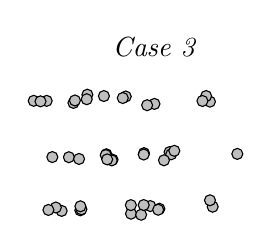
\begin{tikzpicture}[scale=0.7]
  \foreach \i in {1,...,5} {
  \pgfmathsetmacro{\x}{rnd*1.5}
  \pgfmathsetmacro{\y}{rnd*0.2}
  \draw[fill=gray!50] ($(\x,\y)$) circle (0.1);
  }
  \foreach \i in {1,...,5} {
  \pgfmathsetmacro{\x}{rnd*1.5}
  \pgfmathsetmacro{\y}{rnd*0.3}
  \draw[fill=gray!50] ($(\x+1,\y)$) circle (0.1);
  }
  \foreach \i in {1,...,5} {
  \pgfmathsetmacro{\x}{rnd*1.5}
  \pgfmathsetmacro{\y}{rnd*0.3}
  \draw[fill=gray!50] ($(\x+2,\y)$) circle (0.1);
  }
  \foreach \i in {1,...,5} {
      \pgfmathsetmacro{\x}{rnd*1.5}
      \pgfmathsetmacro{\y}{rnd*0.2}
      \draw[fill=gray!50] ($(\x+1+0.5,\y+1)$) circle (0.1);
  }
  \foreach \i in {1,...,5} {
  \pgfmathsetmacro{\x}{rnd*1.5}
  \pgfmathsetmacro{\y}{rnd*0.2}
  \draw[fill=gray!50] ($(\x+2+0.5,\y+1)$) circle (0.1);
  }
  \foreach \i in {1,...,5} {
  \pgfmathsetmacro{\x}{rnd*1.5}
  \pgfmathsetmacro{\y}{rnd*0.1}
  \draw[fill=gray!50] ($(\x+0.5,\y+1)$) circle (0.1);
  }
  \foreach \i in {1,...,5} {
      \pgfmathsetmacro{\x}{rnd*1.5}
      \pgfmathsetmacro{\y}{rnd*0.2}
      \draw[fill=gray!50] ($(\x+1,\y+2)$) circle (0.1);
  }
  \foreach \i in {1,...,5} {
  \pgfmathsetmacro{\x}{rnd*1.5}
  \pgfmathsetmacro{\y}{rnd*0.2}
  \draw[fill=gray!50] ($(\x+2,\y+2)$) circle (0.1);
  }
  \foreach \i in {1,...,5} {
  \pgfmathsetmacro{\x}{rnd*1.5}
  \pgfmathsetmacro{\y}{rnd*0.1}
  \draw[fill=gray!50] ($(\x,\y+2)$) circle (0.1);
  }
  \draw (1.5,3.4)node[below right]{\textit{Case 3}};
\end{tikzpicture}
% \hfill
% \caption{
%   Sketch of the three different particule arrangements identified in this study.
% The gray disks represent droplets in a three-dimensional space.
% Gravity acts in the vertical direction.

% }
% \label{fig:scheme_clusters}
\end{figure}
% \begin{itemize}
%   \item (\textit{Case 1: ``homogeneous''}) A homogeneous arrangement of droplets is called a homogeneous microstructure or just ``homogeneous''.
%   \item (\textit{Case 2: ``clusters''}) Isotropic non-homogeneous microstructure where we observe the presence of ``clusters'' meaning that the particules are close to each other on average.
%   The opposite scenario, where particules are, on average, far from each other, also falls into this category.
%   \item (\textit{Case 3: ``layers''}) The non-isotropic non-homogeneous microstructure where we observe the presence of stratified arrangements.
%   This type of microstructure is referred to as layered microstructure or just ``layers''.
% \end{itemize}
\begin{table}[h!]
  \caption{Microstructure classification}
  \label{tab:microstructure}
  \centering
  \begin{tabular}{|lccccc|} \hline
      Microstructure types & Homogeneous & Isotropic & Figure & $\textbf{R}:\bm\delta/r_m^2$ & $A_{xx}/tr(\textbf{R})$ \\
      Homogeneous & Yes & Yes &(\textit{Case 1}) & $ \approx 1$ & $\approx 0$ \\
      Dispersed &  No & Yes  &(\textit{Case 2}) & $ > 1$ & $\approx 0$ \\
      Clustering &  No & Yes  &(\textit{Case 2}) & $ < 1$ & $\approx 0$ \\
      Layering &    No & No  &(\textit{Case 3}) & $ - $ & $< 1$\\ \hline
  \end{tabular}
\end{table}

\end{frame}


\begin{frame}
  \frametitle{Phase diagram of the microstructure anisotropy}
  \footnotesize
  % \begin{align*}
  %   \textbf{R} = \int \textbf{rr} P_{nst}(\textbf{r}) d\textbf{r}
  %   &&
  %   \textbf{A} = 
  %   \textbf{R} - \frac{1}{3}(\textbf{R}: \bm\delta) \bm\delta
  % \end{align*}
  \begin{figure}[h!]
    \centering
    % \begin{tikzpicture}[scale=0.5]
    %     \node (img) at (0,0) {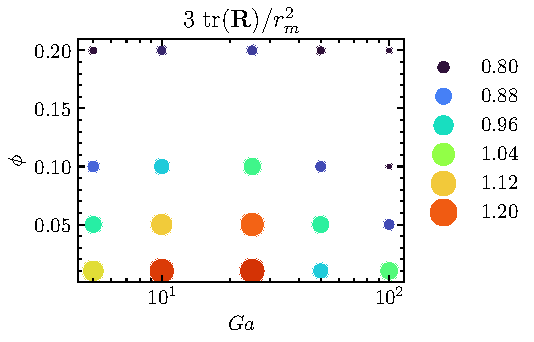
\includegraphics[height=0.3\textwidth]{image/HOMOGENEOUS_NEW/PA/phase_Rtr_l_1.pdf}};
    %     % \draw[dashed] (10cm,-1.6) ellipse (3 and 2);
    %     \node (txt) at (-2,1) {Clustering};
    %     \node (txt) at (-1,-1.6) {Dispersed};
    %     \draw[dashed] ($(-1,-1.6) + (-10:3 and 2)$(P) arc
    %     (-10:155:3 and 2);
    %     \node (img) at (10.5,0) {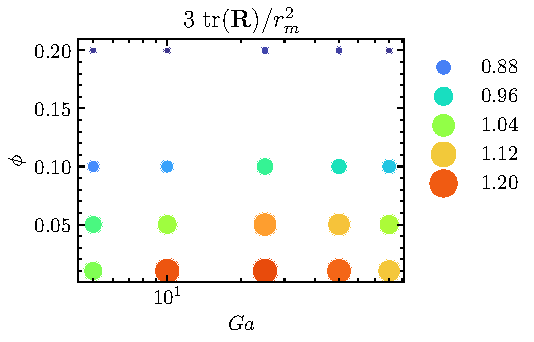
\includegraphics[height=0.3\textwidth]{image/HOMOGENEOUS_NEW/PA/phase_Rtr_l_10.pdf}};
    %     % \draw[dashed] (10cm,-1.6) ellipse (3 and 2);
    %     \node (txt) at (8.5,1) {Clustering};
    %     \node (txt) at (10,-1.6) {Dispersed};
    %     \draw[dashed] ($(10,-2) + (-10:3 and 2)$(P) arc
    %     (-10:180:3 and 2);
    % \end{tikzpicture}
    \begin{tikzpicture}[scale=0.5]
        \node (img) at (0,0) {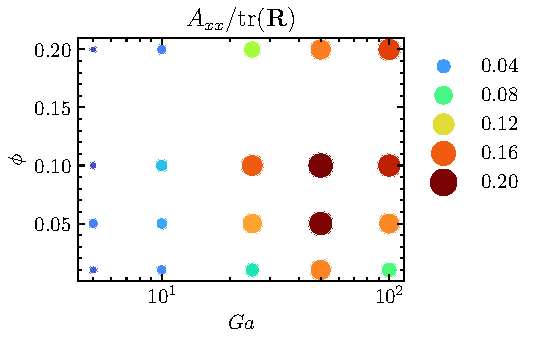
\includegraphics[height=0.3\textwidth]{image/HOMOGENEOUS_NEW/PA/phase_axx_l_1.pdf}};
        \draw[dashed] (1.4,0.3) ellipse (1.5 and 2.5);
        \node (txt) at (1.4,1) {Anisotropic};
        \node (txt) at (-2,1) {Isotropic};

        \node (img) at (10.5,0) {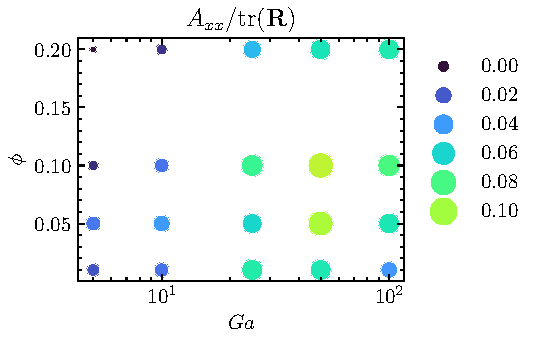
\includegraphics[height=0.3\textwidth]{image/HOMOGENEOUS_NEW/PA/phase_axx_l_10.pdf}};
        % \draw[dashed] (11.7,-0.5) ellipse (0.75 and 1.75);
        % \node (txt) at (11.7,1) {Anisotropic};
        \node (txt) at (8,1) {Isotropic};
    \end{tikzpicture}
    \caption{
        % (top) Phase diagram of the dimensionless mean square distance to the nearest neighbor, $\bm\delta:\textbf{R}/r_m^2$.
         Phase diagram of the dimensionless horizontal components of the anisotropy tensor, $A_{xx}/\text{tr}(\textbf{R})$.  
        (left) Iso-viscosity emulsion $\lambda = 1$.
        (right) Viscous droplets $\lambda = 10$. }
    \label{fig:phase}
\end{figure}

$\to$ Iso-viscosity emulsions exhibit anisotropic clusters at $Ga > 25$ and $\phi \ge 0.05$.  

\end{frame}

\begin{frame}
  {A transport equation to describe the evolution of the microstructure}
  We could show that $\textbf{R}$ obeys the transport equation: 
\begin{equation*}
    \pddt (n_p\textbf{R})
    + \div [
      n_p(\textbf{u}_p\textbf{R}
    + \textbf{R}^\text{Re})]
    = 
    - \frac{n_p\textbf{R}}{\tau_p}
    +n_p\textbf{B}
    + n_p\textbf{D}
    + n_p\textbf{W}
\end{equation*}
With the ``relative velocity production term''
\begin{align*}
    % n_p \textbf{R}^\text{Re}(\textbf{x},t)
    % =
    % \int_{0}^\infty
    % \int_{\mathbb{R}^3}
    % \textbf{rr}(\textbf{u}^\text{nst}_p - \textbf{u}_p)
    % P(\textbf{x},\textbf{r},t,a)
    % d\textbf{r}da,\\
    % n_p \textbf{B}(\textbf{x},t)
    % =
    % \int_{0}^\infty
    % \int_{\mathbb{R}^3}
    % \textbf{rr}
    % P(\textbf{x},\textbf{r},t,0)\delta(a)
    % d\textbf{r}da, \\
    % n_p\textbf{D}(\textbf{x},t) = 
    % \int_{0}^\infty
    % \int_{\mathbb{R}^3} \textbf{rr}
    % \left[
    %     \frac{1}{\tau_p(\textbf{x},t)}
    %     - \frac{1}{\tau^\text{nst}(\textbf{x},\textbf{r},t,a)}
    % \right]
    % P_\text{nst}
    % d\textbf{r}
    % da,\\
    n_p \textbf{W}(\textbf{x},t) = 
    \int_{0}^\infty
    \int_{\mathbb{R}^3} \left[
        \textbf{r} \textbf{w}^\text{nst}_p
        + \textbf{w}^\text{nst}_p\textbf{r}
    \right]P_\text{nst}
    d\textbf{r}
    da.
\end{align*} 

\begin{itemize}
  \item  $\textbf{w}^\text{nst}_p(\textbf{x},\textbf{r},t,a)$ is the averaged relative velocity between two nearest neighboring particules, one of which is situated at $\textbf{x}$ and time $t$, with its nearest neighbor at $\textbf{x}+\textbf{r}$ with age $a$. 
  \item \textbf{R} relaxes on a timescale $\tau_p$ which is related to the particule interaction time.
\end{itemize}

$\to$ The distribution $\textbf{w}^\text{nst}_p$ seems primordial in the evolution of \textbf{R}. 

\end{frame}

\begin{frame}
  \frametitle{DNS statistics for the nearest relative velocity field}

  \begin{figure}[h!]
    \centering
    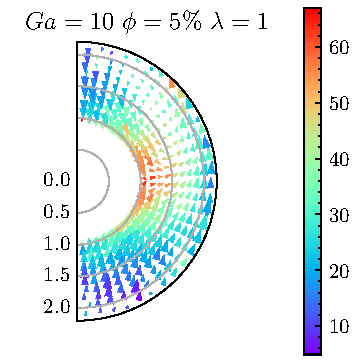
\includegraphics[height=0.35\textwidth]{image/HOMOGENEOUS_NEW/Dist/U_rel_l_1_Ga_10_PHI_5.pdf}
    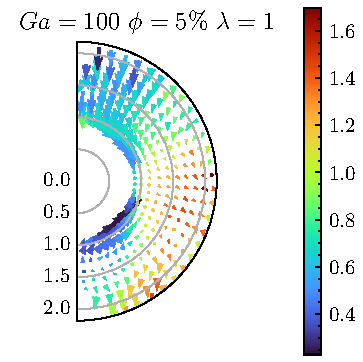
\includegraphics[height=0.35\textwidth]{image/HOMOGENEOUS_NEW/Dist/U_rel_l_1_Ga_100_PHI_5.pdf}
    % \begin{tikzpicture}[scale=0.8]
    %     \filldraw[ gray!50!white](0,0) circle (0.5);
    %     \filldraw[ gray!50!white](1,3)circle (0.5);
    %     \filldraw[ gray!50!white](-0.2,3.5)circle (0.5);
    %     % \draw[fill=gray,opacity=0.2](5,-0.2)circle (0.5);
    %     % \draw[fill=gray,opacity=0.2](-3,2)circle (0.5);
    %     % \draw[fill=gray,opacity=0.2](-5,0.2)circle (0.5);
    %     \draw(0,0)node[right]{$p_1, \; \textbf{x} = 0 $};
    %     \draw[dashed](0,0)--(1,3)node[right]{$p_2, \;\textbf{x}+\textbf{r}$};
    %     \draw[dashed](-0.2,3.5)node[right]{$p_3$};
    % \end{tikzpicture} 
    % 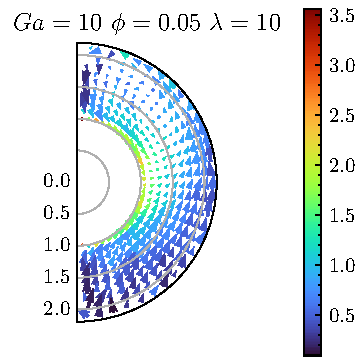
\includegraphics[height=0.35\textwidth]{image/HOMOGENEOUS_NEW/Dist/U_rel_l_10_Ga_10_PHI_5.pdf}
    % 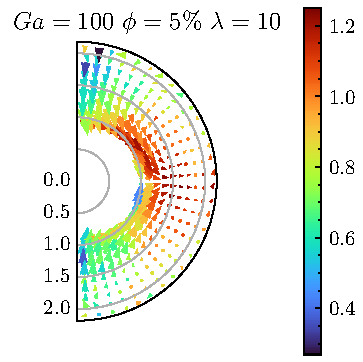
\includegraphics[height=0.35\textwidth]{image/HOMOGENEOUS_NEW/Dist/U_rel_l_10_Ga_100_PHI_5.pdf}
    \caption{
      Quiver plots of the relative averaged velocity field $\textbf{w}^\text{nst}_p(\textbf{x},\textbf{r},t)$ colored by the averaged dimensionless age $a^{nst}(\textbf{x},\textbf{r},t)$ for $\phi = 0.05$ and $\lambda = 1$.
      \break
         (left) $Ga = 10$ (right) $Ga =100$. }
    \label{fig:Why_Ga_matter}
\end{figure}

\begin{itemize}
  \item On average, particules approach vertically and leave through the sides.
  \item Quantitative representation of the Drafting -Kissing-Tumbling mechanism.
\end{itemize}
\end{frame}

\begin{frame}
  {Influence of the viscosity ratio}

  \begin{figure}[h!]
      \centering
      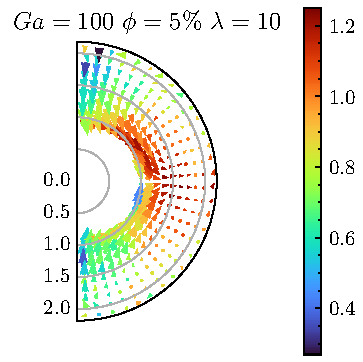
\includegraphics[height=0.35\textwidth]{image/HOMOGENEOUS_NEW/Dist/U_rel_l_10_Ga_100_PHI_5.pdf}
      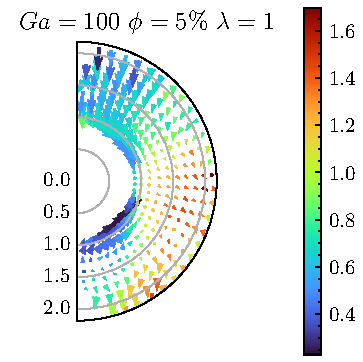
\includegraphics[height=0.35\textwidth]{image/HOMOGENEOUS_NEW/Dist/U_rel_l_1_Ga_100_PHI_5.pdf}
      % 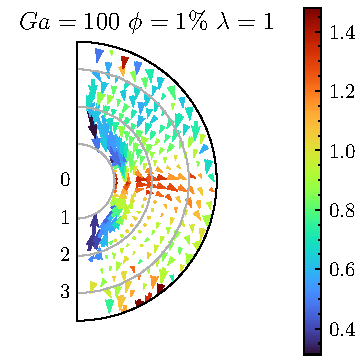
\includegraphics[height=0.35\textwidth]{image/HOMOGENEOUS_NEW/Dist/U_rel_l_1_Ga_100_PHI_1.pdf}
      % 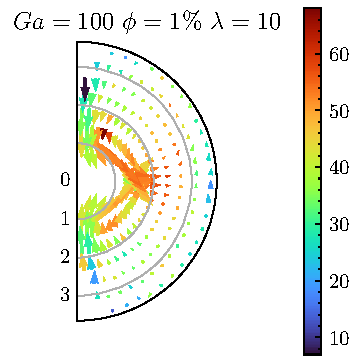
\includegraphics[height=0.35\textwidth]{image/HOMOGENEOUS_NEW/Dist/U_rel_l_10_Ga_100_PHI_1.pdf}
      \caption{Quiver plots of the relative averaged velocity field $\textbf{w}^\text{r}(\textbf{x},\textbf{r},t)$ colored by the averaged dimensionless age $a^r(\textbf{x},\textbf{r},t)$, for $\phi = 0.05$ and $Ga = 100$.
        \break
      (left) High viscosity ratio $\lambda = 10$.
      (right) Low viscosity ratio, $\lambda = 1$. }
      \label{fig:Why_l_matter}
  \end{figure}

  \begin{itemize}
    \item Side-by-side configurations seem more stable for $\lambda = 1$ which explains partly the form of $P_{nst}(\textbf{r})$. 
  \end{itemize}
\end{frame}

% \begin{frame}
%   \frametitle{Nearest averaged flow fields around a particule}
% \begin{figure}[h!]
%   \centering
%   \begin{tikzpicture}
%       \node (img) at (0,0)  {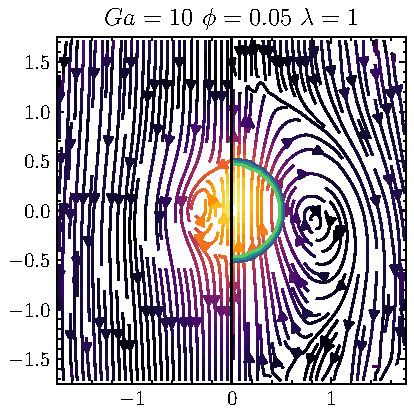
\includegraphics[height=0.25\textwidth]{image/HOMOGENEOUS/Stream/Stream_PHI_5_Ga_10_l_1.pdf}};
%       \node (img) at (0.25\textwidth,0)  {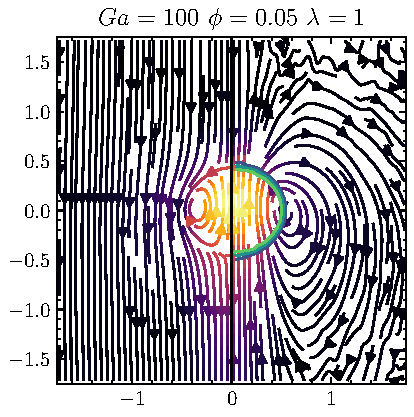
\includegraphics[height=0.25\textwidth]{image/HOMOGENEOUS/Stream/Stream_PHI_5_Ga_100_l_1.pdf}};
%       \node (img) at (0.5\textwidth,0)  {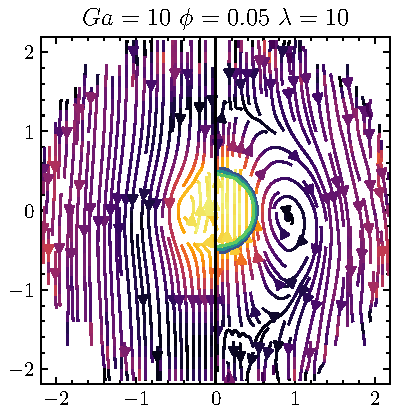
\includegraphics[height=0.25\textwidth]{image/HOMOGENEOUS/Stream/Stream_PHI_5_Ga_10_l_10.pdf}};
%       \node (img) at (0.75\textwidth,0)  {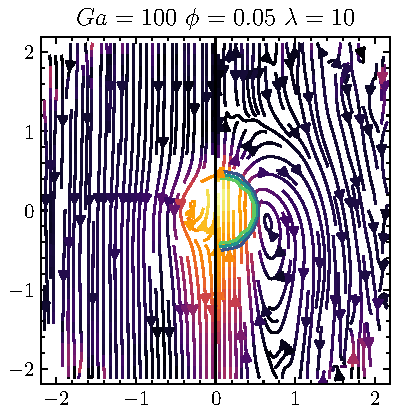
\includegraphics[height=0.25\textwidth]{image/HOMOGENEOUS/Stream/Stream_PHI_5_Ga_100_l_10.pdf}};
%   \end{tikzpicture}
%   \caption{Nearest particule averaged velocity $\nstavg{\textbf{u}}(\textbf{r})$ for  $\phi = 5\%$ and $20\%$.
%   Green lines : contour plots of the nearest averaged indicator function $\nstavg{\chi_d}(\textbf{r})$ (it represent the mean shape of the particules)}
%   \label{fig:Stream}
% \end{figure}

% \begin{itemize}
%   \item Hill vortex inside the particule = closure for mathematical model
%   \item $\lambda = 1 \rightarrow$ bubbles wake condition.
%   ; $\lambda = 10 \rightarrow$ solid particule wake condition. 
% \end{itemize}
% \end{frame}

\section{Conclusion and perspectives}
\section*{}

\begin{frame}
  \frametitle{Conclusion and perspectives}

  \begin{itemize}
    \item We used the Nearest Particule Statistics framework to describe the microstructure of dispersed two-phase flow. 
    \item We could show that the microstructure can be described qualitatively and quantitatively using the second-order tensor \textbf{R}.
    \item An averaged evolution equation for this tensor was derived.
    \item The viscosity ratio $\lambda$ has a strong impact on the microstructure. 
    % \item We used the nearest particule statistics to derive relative pair interactions equations. 
    % \item We found out that relative positions and velocity were directly correlated to the relative position \textbf{r} and age of the interaction $a$, with $Ga$ and $\phi$. and $\lambda$ 
      % \item The interaction relaxation time corresponds approximately to the mean age of interaction $\tau =\avg{a}$.
    \item Paper to appear in a special issue of Acta Mechanica.
  \end{itemize}
\vfill    
% \vspace{1cm}
See Nicolas' work here: \url{http://basilisk.fr/sandbox/fintzin/Rising-suspension/RS.c}

\end{frame}


 
\backmatter

\begin{frame}
  \frametitle{DNS statistics for the nearest relative velocity field}
  \begin{figure}
      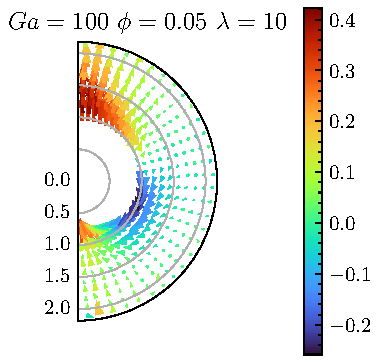
\includegraphics[height=0.35\textwidth]{image/HOMOGENEOUS_NEW/Dist/U_l_10_Ga_100_PHI_5.pdf}
      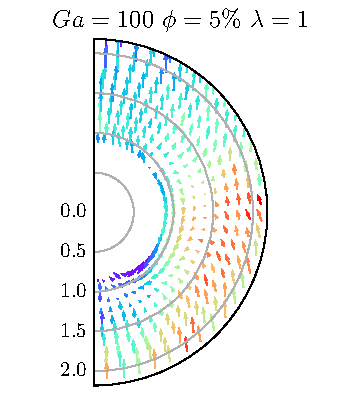
\includegraphics[height=0.35\textwidth]{image/HOMOGENEOUS_NEW/Dist/U_l_1_Ga_100_PHI_5.pdf}
    % \includegraphics[height=0.35\textwidth]{image/HOMOGENEOUS_NEW/Dist/U_l_1_Ga_10_PHI_5
    \caption{ Nearest averaged particule center of mass velocity fields, $(\textbf{u}_p^{nst} (\textbf{r},a) - \textbf{u}_p) / \textbf{u}_p$
    Colormap : dimensionless age of interaction $a$. }
  \end{figure}

\begin{itemize}
  \item ($\lambda = 10$) Isolated particules are \underline{slower} than the mean velocity $\textbf{u}_p$.
  \item ($\lambda = 1$) Isolated particules are \underline{faster} than the mean velocity $\textbf{u}_p$.
\end{itemize}

\end{frame}

\begin{frame}
  \frametitle{Representation of the interaction force}

  \begin{figure}
    % 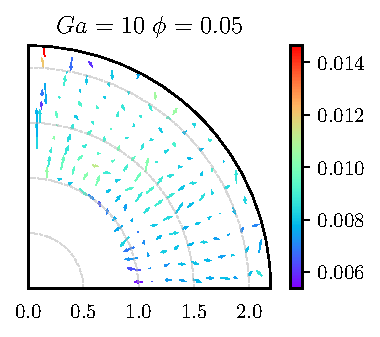
\includegraphics[height=0.25\textwidth]{image/HOMOGENEOUS/fDrop/F_mu_r_0_1_Ga_10_PHI_0_05.pdf}
    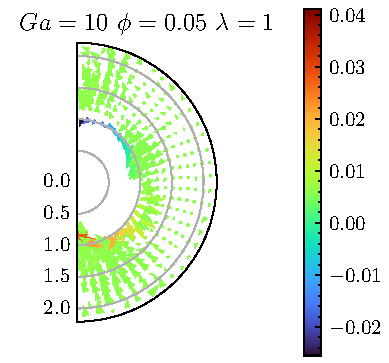
\includegraphics[height=0.25\textwidth]{image/HOMOGENEOUS_NEW/Dist/F_rel_l_1_Ga_10_PHI_5.pdf}
    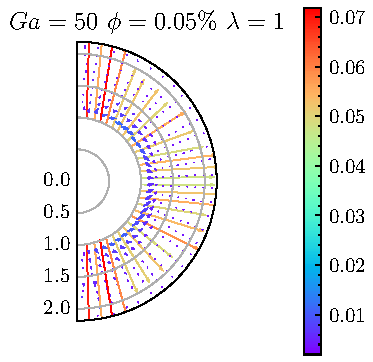
\includegraphics[height=0.25\textwidth]{image/HOMOGENEOUS_NEW/Dist/F_rel_l_1_Ga_50_PHI_5.pdf}
    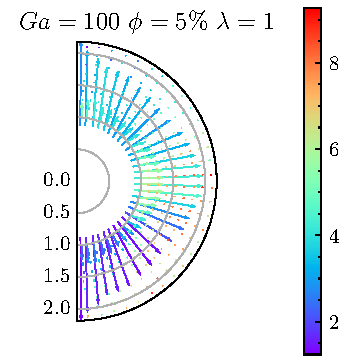
\includegraphics[height=0.25\textwidth]{image/HOMOGENEOUS_NEW/Dist/F_rel_l_1_Ga_100_PHI_5.pdf}
    
    \caption{Nearest averaged relative acceleration fields times the mass of a particule $\nstavg{\textbf{f}}(\textbf{r},a)$. 
    Color map : Dimensionless age of the interaction.}
  \end{figure}

  
\begin{itemize}
  % \item $\nstrelavg{\textbf{F}}$ is an isotropic repulsion force at high $Ga$. 
  % \item At lower $Ga$ we observe attraction forces $\nstrelavg{\textbf{F}}$ on the sides.
  \item The force is always repulsive on the vertical direction.  
  \item On the sides  directions, Long time interactions results into attraction forces, while short time interaction into repulsion forces.
  \item Attraction forces might lead to coalesence. 
\end{itemize}

$\rightarrow$ How to quantify these fields ? 
\end{frame}





\begin{frame}
  \frametitle{Computation of the Particule Fluid Particule (PFP) stress}
  \underline{What is the particule stress (Zhang, JFM, 2021) ?}  
   : $\avg{\text{Drag Force}} = \avg{F} + \div \Sigma_{PFP}$
  \begin{figure}
    % 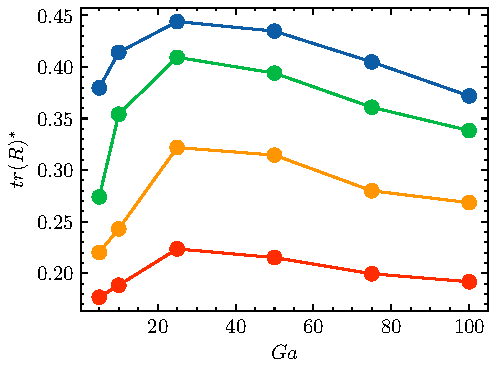
\includegraphics[height=0.23\textwidth]{image/HOMOGENEOUS/fPA/RR.pdf}
    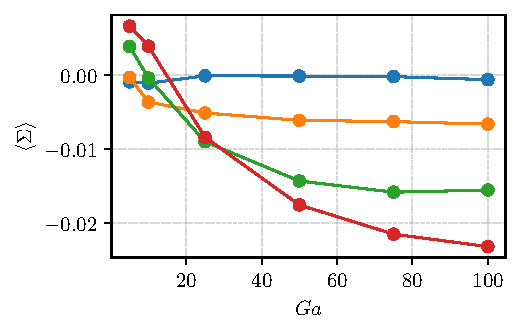
\includegraphics[height=0.23\textwidth]{image/HOMOGENEOUS/fPA/PFP.pdf}
    \caption{ 
      % (left) Dimensionless  mean square distance to the nearest neighbor ($\textbf{R}^* =0$ particule in contact). 
      (right) Particule fluid particule stress $\mathbf{\Sigma}_{PFP} = \int \textbf{r}\nstavg{\textbf{f}} P_{nst}d\textbf{r}$.
      }
  \end{figure}
  
\begin{itemize}
  \item $\text{tr}(\mathbf{\Sigma}_{PFP}) > 0$ global repulsion for high $\phi$ and $Ga$. 
  \item $\text{tr}(\mathbf{\Sigma}_{PFP}) < 0$ global attraction for small $Ga$ and $\phi$.
  % \item $\text{tr}(\mathbf{\Sigma}_{PFP}) = 0$ no pressure, when $\phi \rightarrow 0$ and $Ga \rightarrow 0$. 
  \item  $\mathbf{\Sigma}_{PFP}$ is then correlated with the mean nearest particule distance $\mathbb{R}$. 
\end{itemize}

\end{frame}


\begin{frame}
  \frametitle{Distribution of the interaction time between a pair of the nearest particule}
    \begin{figure}
        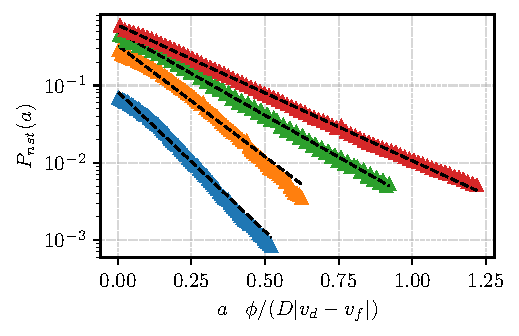
\includegraphics[height=0.23\textwidth]{image/HOMOGENEOUS/fDrop/P_a_Ga_25.pdf}
        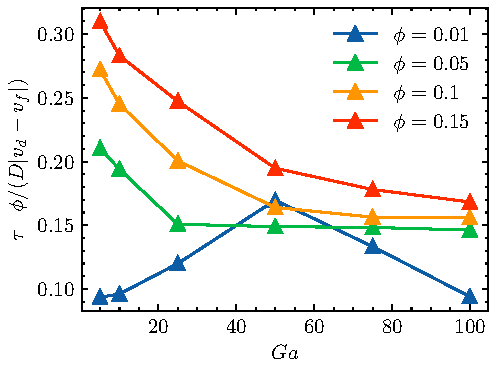
\includegraphics[height=0.23\textwidth]{image/HOMOGENEOUS/fPA/ageGa.pdf}
        \caption{ (left) PDF of the dimensionless age of interaction for fixed $Ga = 25$.
      (right) Mean time of interaction $\tau(\textbf{x})$.}
    \end{figure}
  \begin{equation*}
    P_{nst}(\textbf{x},a) 
    = \int P_{nst}(\textbf{x},\textbf{r},\textbf{w},a) d\textbf{w}d\textbf{r}
    \rightarrow\frac{e^{-a/\tau(\textbf{x})}}{\tau(\textbf{x})}
  \end{equation*}
\begin{itemize}
  \item $\tau(\textbf{x}) = \int a P_{nst}(\textbf{x},a) da$ is the mean interaction time at $\textbf{x}$. 
\end{itemize}
\end{frame}

\begin{frame}
  \frametitle{On the way to model the coalescence kernel}
    \begin{figure}
        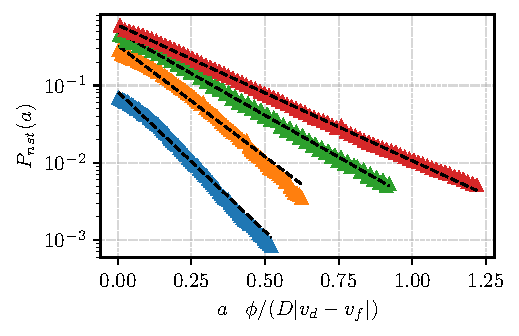
\includegraphics[height=0.23\textwidth]{image/HOMOGENEOUS/fDrop/P_a_Ga_25.pdf}
        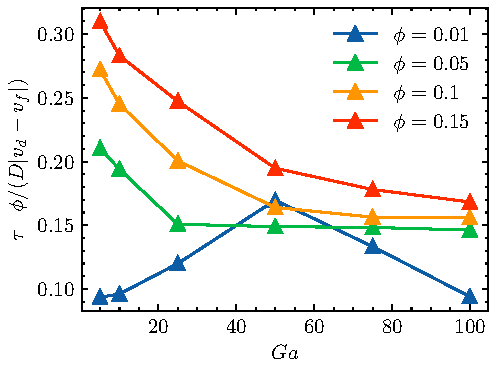
\includegraphics[height=0.23\textwidth]{image/HOMOGENEOUS/fPA/ageGa.pdf}
        \caption{ (left) PDF of the dimensionless age of interaction for fixed $Ga = 25$.
      (right) Mean time of interaction $\tau(\textbf{x})$.}
    \end{figure}
  \textbf{For coalescence modeling : }
\begin{itemize}
  \item Rate of coalescence : $\int_{a > t_c}^\infty P_{nst}(\textbf{x},t,a) da 
  = \frac{e^{-t_c/\tau(\textbf{x})}}{\tau(\textbf{x})}$. 
  \item $t_c$ is the critical time of coalescence determined by the film drainage problem (Paul-Peter Phd)
\end{itemize}

\end{frame}




% \section{Evolution of interactions dynamics}

\section*{}

\begin{frame}
  \frametitle{Let study the interaction time between  a pair of the nearest particule}
    \begin{figure}
        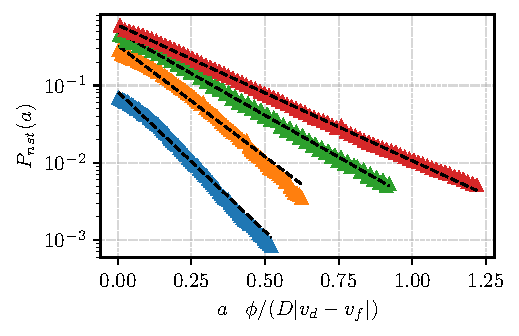
\includegraphics[height=0.23\textwidth]{image/HOMOGENEOUS/fDrop/P_a_Ga_25.pdf}
        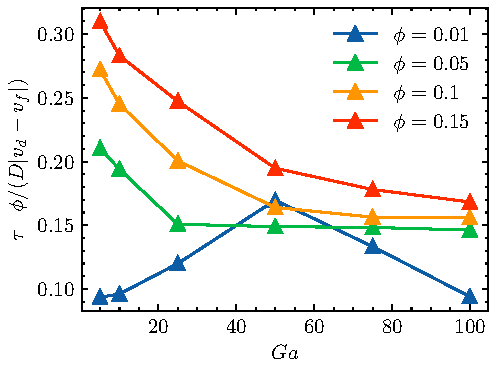
\includegraphics[height=0.23\textwidth]{image/HOMOGENEOUS/fPA/ageGa.pdf}
        \caption{ (left) PDF of the dimensionless age of interaction for fixed $Ga = 25$.
      (right) Mean time of interaction $\tau(\textbf{x})$.}
    \end{figure}
  \begin{equation*}
    P_{nst}(\textbf{x},a) 
    = \int P_{nst}(\textbf{x},\textbf{r},\textbf{w},a) d\textbf{w}d\textbf{r}
    \rightarrow\frac{e^{-a/\tau(\textbf{x})}}{\tau(\textbf{x})}
  \end{equation*}
\begin{itemize}
  \item $\tau(\textbf{x}) = \int a P_{nst}(\textbf{x},a) da$ is the mean interaction time at $\textbf{x}$. 
\end{itemize}
\end{frame}

\begin{frame}
  \frametitle{Position history of the interaction}
    \begin{figure}
        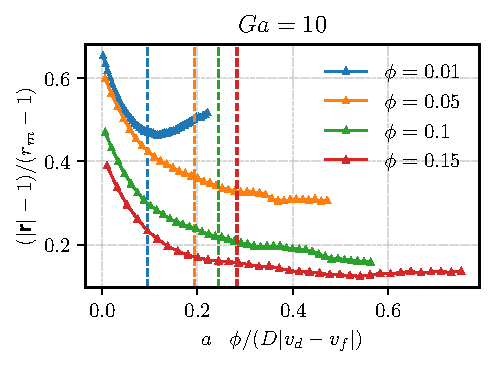
\includegraphics[height=0.23\textwidth]{image/HOMOGENEOUS/fDrop/r_a_Ga_10.pdf}
        \includegraphics[height=0.23\textwidth]{image/HOMOGENEOUS/fDrop/r_a_Ga_75.pdf}
        \caption{ Conditional average $\nstavg{\textbf{r}}(a)$ on the age of the interaction} 
    \end{figure}
  \begin{equation*}
     \nstavg{\textbf{r}}(\textbf{x},a)
    = e^{a/\tau(\textbf{x})}\tau(\textbf{x})\int \textbf{r} P_{nst}(\textbf{x},\textbf{r},\textbf{w},a) d\textbf{w}d\textbf{r}
    % = \frac{e^{-a/\tau(\textbf{x})}}{\tau(\textbf{x})}
  \end{equation*}

\end{frame}

\begin{frame}
  \frametitle{Velocity fluctuations}
  \begin{figure}[h!]
    \centering
    \begin{tikzpicture}
        \node (img) at (0.3\textwidth,-0.6\textwidth)  {\includegraphics[height=0.3\textwidth]{image/HOMOGENEOUS/Stream/P_PHI_5_Ga_50_l_1.pdf}};
        \node (img) at (0.6\textwidth,-0.6\textwidth)  {\includegraphics[height=0.3\textwidth]{image/HOMOGENEOUS/Stream/P_PHI_5_Ga_100_l_1.pdf}};
    \end{tikzpicture}
    \caption{Nearest particule averaged pressure $\nstavg{p}(\textbf{r})$ normalized by the Laplace pressure $4 \gamma /d$ for  $\phi = 5\%$ and $20\%$}  
    \label{fig:Stream}
\end{figure}
  

\end{frame}

\begin{frame}
  \frametitle{Kinematic history of the interaction}
    \begin{figure}
        \includegraphics[height=0.24\textwidth]{image/HOMOGENEOUS/fDrop/ur_a_Ga_5.pdf}
        \includegraphics[height=0.24\textwidth]{image/HOMOGENEOUS/fDrop/ur_a_Ga_75.pdf}
        \caption{Conditional average of the normal relative velocity : $\nstavg{\textbf{w}_n}(a) = \nstavg{\textbf{w}}(a)\cdot \textbf{r}/|\textbf{r}|$ for $Ga = 5,100$ in terms of the dimensionless age $a$.
        (dashed lines) average time of interaction, $\tau(\textbf{x})$}. 
    \end{figure}
  \begin{equation*}
     \nstavg{\textbf{w}_n}(\textbf{x},a)
    = e^{a/\tau(\textbf{x})}\tau(\textbf{x})\int \textbf{w}\cdot(\textbf{r}/|\textbf{r}|) P_{nst}(\textbf{x},\textbf{r},\textbf{w},a) d\textbf{w}d\textbf{r}
    % = \frac{e^{-a/\tau(\textbf{x})}}{\tau(\textbf{x})}
  \end{equation*}

$\rightarrow$ $\tau(\textbf{x},a)$ correspond roughly to the relaxation time of $\nstavg{\textbf{w}_n}(\textbf{x},a)$
\end{frame}
\begin{frame}
  \frametitle{Dynamics history of the interaction}
    \begin{figure}
      \includegraphics[height=0.24\textwidth]{image/HOMOGENEOUS/fDrop/f_a_Ga_5.pdf}
      \includegraphics[height=0.24\textwidth]{image/HOMOGENEOUS/fDrop/f_a_Ga_75.pdf}
        \caption{Conditional average of the normal relative forces : $\nstavg{\textbf{f}_n}(a) = \nstavg{\textbf{f}}(a)\cdot \textbf{r}/|\textbf{r}|$ for $Ga = 5,10$ . 
        (dashed lines) avenged time of interaction, $\tau(\textbf{x})$}. 
    \end{figure}

\begin{itemize}
  \item $\tau(\textbf{x})$ correspond also to the relaxation of $\nstavg{\textbf{f}_n}(\textbf{x},a)$
  \item For $a > \tau(\textbf{x})$ we roughly have $\nstavg{\textbf{f}_n}(\textbf{x},a) \leq 0 $
\end{itemize}
$\rightarrow$After a time of interaction of $a \geq \tau$ the force is relatively low or attractive,  and the relative velocity is constant. 
\end{frame}


\begin{frame}
  \frametitle{Conditional average of the force on the velocity}
  \begin{figure}
    \centering
    \includegraphics[width=0.33\textwidth]{image/HOMOGENEOUS/fDrop/F_mu_r_0_1_Ga_25_PHI_0_05.pdf}
    \includegraphics[width=0.33\textwidth]{image/HOMOGENEOUS/fDrop/Fpos_mu_r_0_1_Ga_25_PHI_0_05.pdf}
    \includegraphics[width=0.33\textwidth]{image/HOMOGENEOUS/fDrop/Fneg_mu_r_0_1_Ga_25_PHI_0_05.pdf}
    \caption{Nearest averaged force fields, $\nstrelavg{\textbf{F}}(\textbf{r})$ for different $Ga$ and $\phi$. 
    Color map : Magnitude of the dimensionless force  $\nstrelavg{\textbf{F}} / (\Delta \rho V g)$.
    (middle) conditional average  $\nstrelavg{\textbf{F}| u_r > 0}(\textbf{r})$. 
    (right) conditional average  $\nstrelavg{\textbf{F}| u_r < 0}(\textbf{r})$ }
  \end{figure}
\end{frame}

\begin{frame}
  \frametitle{Conditional average of the force on the velocity}
  \begin{figure}
    \centering
    \includegraphics[width=0.33\textwidth]{image/HOMOGENEOUS/fDrop/F_mu_r_0_1_Ga_5_PHI_0_05.pdf}
    \includegraphics[width=0.33\textwidth]{image/HOMOGENEOUS/fDrop/Fpos_mu_r_0_1_Ga_5_PHI_0_05.pdf}
    \includegraphics[width=0.33\textwidth]{image/HOMOGENEOUS/fDrop/Fneg_mu_r_0_1_Ga_5_PHI_0_05.pdf}
    \caption{Nearest averaged force fields, $\nstrelavg{\textbf{F}}(\textbf{r})$ for different $Ga$ and $\phi$. 
    Color map : Magnitude of the dimensionless force  $\nstrelavg{\textbf{F}} / (\Delta \rho V g)$.
    (middle) conditional average  $\nstrelavg{\textbf{F}| u_r > 0}(\textbf{r})$. 
    (right) conditional average  $\nstrelavg{\textbf{F}| u_r < 0}(\textbf{r})$ }
  \end{figure}
\end{frame}






\end{document}
